\chapter{予備実験について}
本付録では,本研究の予備実験に行われた実験手法及び評価に関する詳細を表記する.
  \section{アプローチ}
\subsection{行動予測の記録}
総所要予測時間,必要タスク予測,タスク別所要時間予測を申告してもらった.尚,総所要予測時間は支度開始見込み時刻と外出理想時刻(第一理想時刻),外出時刻のタイムリミット(第二理想時刻)を申告してもらい,支度開始見込時刻を差し引く事で総所要予測時刻を計算した.
\subsection{因子の評価}
心理的時間による変動の影響を調査する為,前日と当日に,体調,疲労度,ストレス,眠気,モチベーション,予定のルーティン化を5段階で評価してもらう.また,睡眠時間も記録する.
\subsection{実測行動の記録}
ADLogger(4章参照)を用い,当日の外出準備遂行時にADLの記録を実施する.
遂行タスクをtodoリスト形式で事前登録を行ってもらう.当日の外出準備の際には各タスク開始時及び終了時に各リスト脇にあるストップウォッチを操作してもらう事でタスク別の所要時間を記録する.

\section{評価実験}
\subsection{実験概要}
被験者実験に関しては,時間管理の苦手意識の有無でグループ分けを行った上で,所要時間の予測/実測の比較及び心理的時間の変動因子の関連性を調査した.実験期間は7日間とし,慶應義塾大学生9名に協力頂いた,内,時間管理に対し苦手意識のある被験者は6名だった,
\subsection{実験結果}
実験期間中に実験データが取得できたのは3名(内苦手意識のある被験者1名)だった.以後被験者A,B,C,と供述する.被験者データとしては被験者Aのみ苦手意識があり.被験者Bのみ3日間,それ以外が1日間のデータが得られた,日常生活動作において被験者A,B,Cは最大3分以上認識の誤差が生じていた.両者グループを比較した際は,Aの方がより誤差の範囲が大きかった.
\begin{figure}[ht]
\begin{center}
\begin{tabular}{c}

	\begin{minipage}[b]{0.5\linewidth}
	\begin{center}
		\fbox{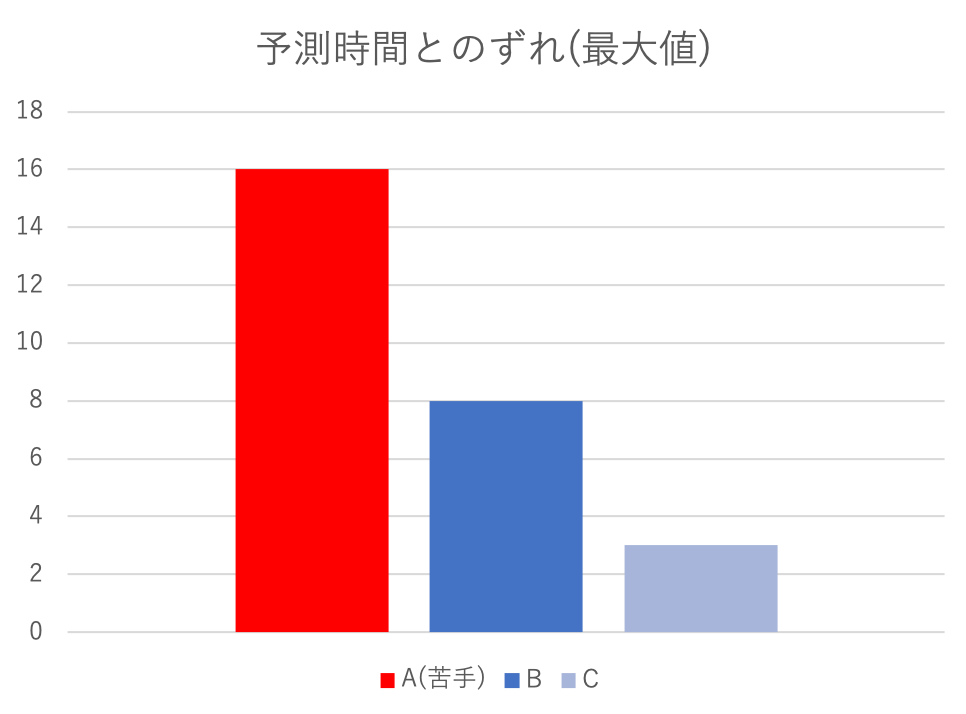
\includegraphics[width=8cm]{images/append/1.png}}
		\caption{被験者結果1}
		\label{fig:top_point}
	\end{center}
  	\end{minipage}
	
		\begin{minipage}[b]{0.5\linewidth}
	\begin{center}
		\fbox{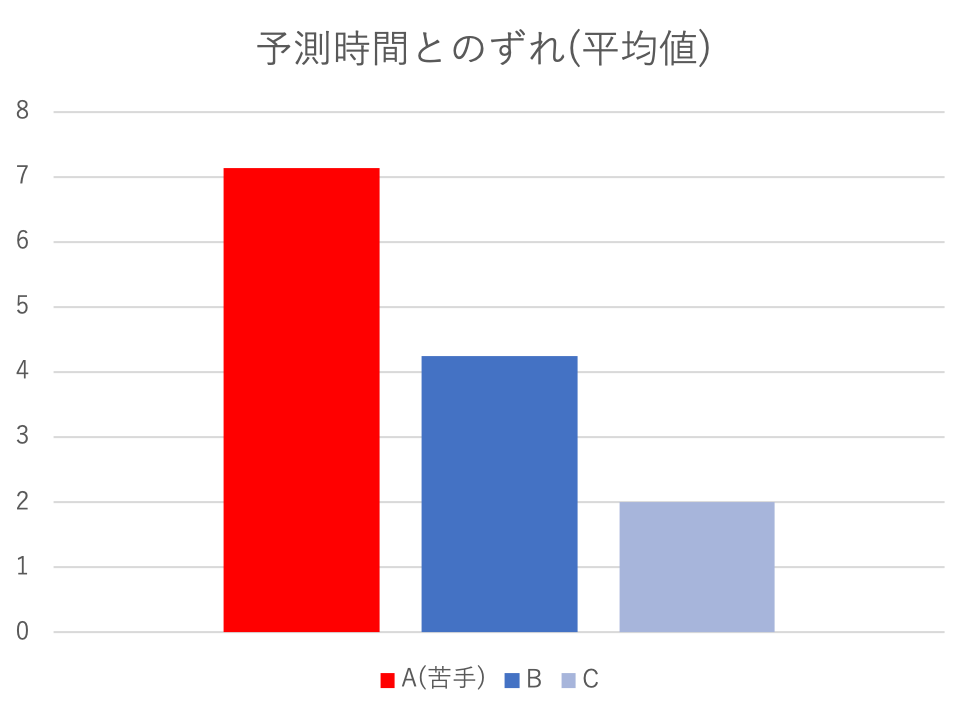
\includegraphics[width=8cm]{images/append/2.png}}
		\caption{被験者結果2}
		\label{fig:top_point}
	\end{center}
  	\end{minipage}

\end{tabular}
\end{center}
\end{figure}

誤差が生じる項目としては日毎にずれる事が多かったものの,歯磨き,化粧,食事と言った項目で誤差の生みやすい傾向が見られた.また,被験者によっては時間の計画の時点から不備が発生している日もあった.Bにおいては日常生活動作毎の予測時間の合計が予想準備時間(支度開始見込み時刻 - 第一理想時刻)を超えており,計画面から間に合わない計画を立てていた.(事実その日は第一理想時刻には間に合わず,第一理想時刻と第二理想時刻の間に外出していた.)また,それぞれの日常生活動作の内訳及び五段階評価に関する結果は以下の通りである.
\begin{figure}[ht]
\begin{center}
\begin{tabular}{c}

	\begin{minipage}[b]{0.5\linewidth}
	\begin{center}
		\fbox{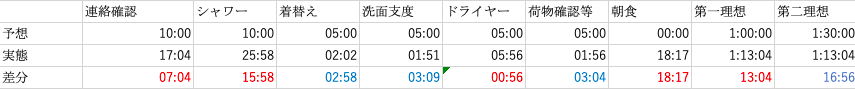
\includegraphics[width=12cm]{images/append/A1.png}}
		\caption{被験者Aの内訳}
		\label{fig:top_point}
	\end{center}
  	\end{minipage}
\\
			\begin{minipage}[b]{0.5\linewidth}
	\begin{center}
		\fbox{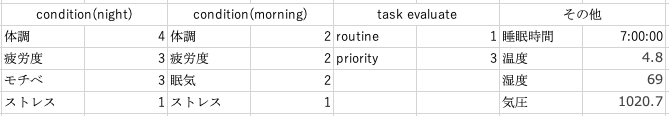
\includegraphics[width=12cm]{images/append/A2.png}}
		\caption{被験者Aの五段階評価}
		\label{fig:top_point}
	\end{center}
  	\end{minipage}
\\
	\begin{minipage}[b]{0.5\linewidth}
	\begin{center}
		\fbox{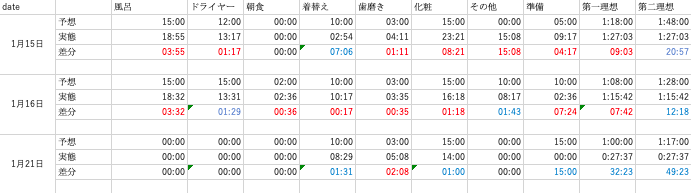
\includegraphics[width=12cm]{images/append/B1.png}}
		\caption{被験者Bの内訳}
		\label{fig:top_point}
	\end{center}
  	\end{minipage}
\\
	\begin{minipage}[b]{0.5\linewidth}
	\begin{center}
		\fbox{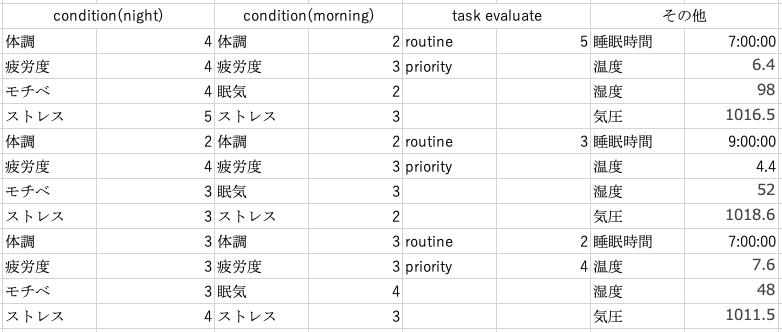
\includegraphics[width=12cm]{images/append/B2.png}}
		\caption{被験者Bの五段階評価}
		\label{fig:top_point}
	\end{center}
  	\end{minipage}
\\
	\begin{minipage}[b]{0.5\linewidth}
	\begin{center}
		\fbox{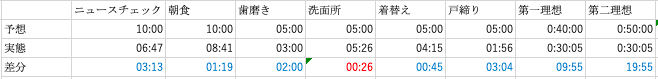
\includegraphics[width=12cm]{images/append/C1.png}}
		\caption{被験者Cの内訳}
		\label{fig:top_point}
	\end{center}
  	\end{minipage}
\\
	\begin{minipage}[b]{0.5\linewidth}
	\begin{center}
		\fbox{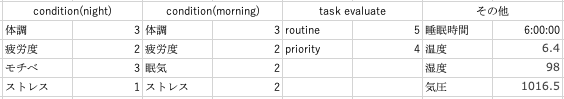
\includegraphics[width=12cm]{images/append/C2.png}}
		\caption{被験者Cの五段階評価}
		\label{fig:top_point}
	\end{center}
  	\end{minipage}
\\
\end{tabular}
\end{center}
\end{figure}

\subsection{考察}
被験者データが集まらなかった理由としては,\UTF{2460}試験期間による外出日の減少 \UTF{2461}実験データが端末保存だった \UTF{2462}実験期間中被験者が記録を忘れた \UTF{2463}実験期間中被験者が記録を忘れた点が原因であると考えられる.
また,計画の時点で破綻したデータがあった為,「逆算が苦手」の定義は各タスク見込み時間を実態より短く認識している」場合と「タスク見込み時間の総時間と総準備時間の認識が合致しておらず,逆算の構造化がなされていない」場合が考えられる.更に破綻したデータは苦手意識のないグループで発見された為,本人の苦手意識にか関わらず被験者の時間管理能力を把握していく必要があると考えられる.

5段階評価との関連性に関しては,「体調・疲労度・優先度・温度・気圧」辺りを中心に相関性が得られる可能性がある.本研究の予備実験として引き続きデータ収集を行いたい.また,有用性に関するインタビューでは「朝に記録し継続する事に対する難しさ」を指摘する声が多かった為,現時点での有用性は十分では無く,更なる改善が必要であると考えられる.